%%%%% Magnetisches Feld %%%%%
%% Massenspektrometer %%


%Some sample text to be displayed above the first subsection

%\subsection{Prinzip}

%Ein Zyklotron besteht aus Zwei hohlen, halbzylindrischen und Duanden an denen eine Spannung mit unterschiedlichem Vorzeichen anliegt, und darüber bzw. darunter liegende Magneten, die ein homogenes Magnetfeld erzeugen. Zudem gibt es einen Einlass und einen Auslass für Teilchen.

%\begin{wrapfigure}{r}{0.4\textwidth} \label{Zyklo}
%
%	\vspace{-10pt}
%	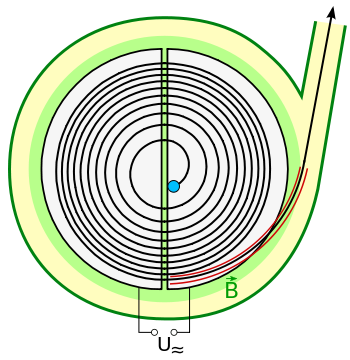
\includegraphics[width=0.35\textwidth]{Zyklotron_Prinzipskizze02.png}
%	\vspace{-13pt}
%	\caption{Prinzipskizze eines Zyklotrons}
%	\vspace{-5pt}	
%	
%\end{wrapfigure}

%\subsubsection{Anwendung}

% Some Formula:

%\begin{equation}
%	x= \frac{y \cdot 13 \pi z}
%			{\cos \alpha}
%\end{equation}

%%%%%%%%%%%%%%%%%%%%%%%
% Eigentlicher Beginn %
%%%%%%%%%%%%%%%%%%%%%%%

Das Massenspektrometer macht man sich zur Identifikation von chemischen Elementen und deren Isotopen die unterschiedlichen Atommassen zu Nutze. Die ersten funktionstüchtigen Massenspektrometer gibt es seit dem frühen 20. Jahrhundert.

\subsection{Aufbau}

In der Ionenquelle werden Atome aus der Probe gelöst und ionisiert. Das heißt, sie sind nun im gasförmigen Zustand und zudem positiv geladen.

Nach einer Beschleunigungseinheit und einem Wien'schen Filter werden sie in ein homogenes Magnetfeld geleitet in welchem sie dann, gemäß der Lorentzkraft auf eine Kreisbahn gezwungen werden. 

Da man absolute Gewissheit über Ladung, Geschwindigkeit hat und auch die Flussdichte des Magnetfeldes kennt, ist die einzige Variable, die den Auftreffpunkt auf der Indikatorplatte bestimmt, die Masse des Atoms. Wie beim Fadenstrahlrohr (Siehe \referenz{sec:Fadenstrahlrohr}) wird der Ansatz $F_{Zp} = F_{Lr}$ vollzogen:

\begin{align}
\begin{split}
	F_{Zp} 				  &= F_{Lr} \\
	m \cdot \frac{v^2}{r} &= q \cdot B \cdot v \\
	m 					  &= \frac{q \cdot B \cdot r}{v}
\end{split}
\end{align}










